% !TeX root = ../Book1.tex
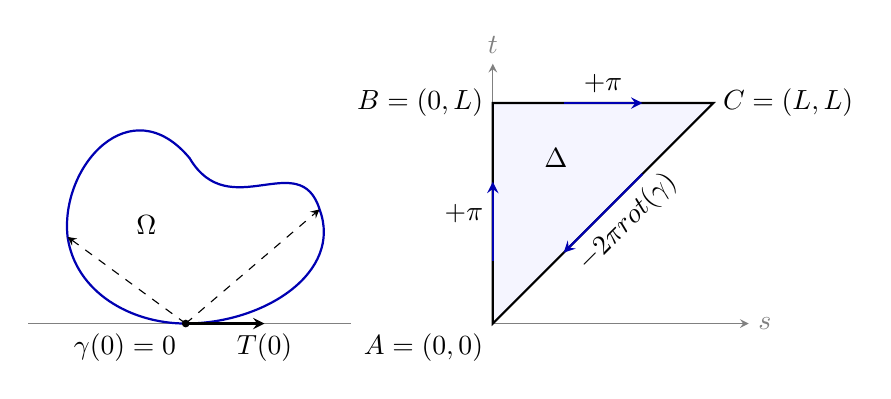
\begin{tikzpicture}[x=1cm,y=1cm,>=stealth]
	\begin{scope}[shift={(1.7,0.25)}]
		\draw[gray] (-2,0)--(2.1,0);
		\draw[thick,blue!70!black] (0,0) .. controls (1,0) and (2,0.65) .. (1.7,1.45) .. controls (1.45,2.25) and (0.55,1.25) .. (0.05,2.1) .. controls (-0.7,3) and (-1.6,2) .. (-1.5,1.1) .. controls (-1.4,0.4) and (-0.7,0) .. (0,0);
		\draw[->,thick] (0,0)--(1,0) node[below] {\(T(0)\)};
		\draw[dashed,->] (0,0)--(1.7,1.45);
		\draw[dashed,->] (0,0)--(-1.5,1.1);
		\fill (0,0) circle (1.4pt);
		\node[below left] at (0,0) {\(\gamma(0)=0\)};
		\node at (-0.5,1.25) {\(\Omega\)};
	\end{scope}
	\begin{scope}[shift={(5.6,0.25)}]
		\fill[blue!4] (0,0)--(0,2.8)--(2.8,2.8)--cycle;
		\draw[->,gray] (0,0)--(3.25,0) node[right] {\(s\)};
		\draw[->,gray] (0,0)--(0,3.3) node[above] {\(t\)};
		\draw[thick] (0,0)--(0,2.8)--(2.8,2.8)--cycle;
		\draw[->,blue!70!black,thick] (0,0.8)--(0,1.8);
		\draw[->,blue!70!black,thick] (0.9,2.8)--(1.9,2.8);
		\draw[->,blue!70!black,thick] (1.9,1.9)--(0.9,0.9);
		\node[left] at (0,1.4) {\(+\pi\)};
		\node[above] at (1.4,2.8) {\(+\pi\)};
		\node[rotate=45,below] at (1.5,1.5) {\(-2\pi\operatorname{rot}(\gamma)\)};
		\node at (0.8,2.1) {\(\Delta\)};
		\node[below left] at (0,0) {\(A=(0,0)\)};
		\node[left] at (0,2.8) {\(B=(0,L)\)};
		\node[right] at (2.8,2.8) {\(C=(L,L)\)};
	\end{scope}
\end{tikzpicture}
